\subsubsection{Typ}
Java-klass

\subsubsection{Syfte}
På serversidan kommer olika delar kombineras för att generera en video som visar användarens test av applikationen. Rörelsehändelserna kommer representeras i form utav en text-fil med data. När videon sedan renderas kommer denna data användas för att rita ut rörelsehändelserna. \\
Komponenten ämnar uppfylla kravet ``Realtidsfingerrörelser'' (Se 3.2.4, URD-1).

\subsubsection{Funktionalitet}
När en inspelning startar börjar mobilen spara varje rörelsehändelse. Denna information sparas till en fil enligt JSON-standard. Exempel på den information som sparas är: \\
\begin{verbatim}
{timestamp=''1000'', interval=''17'', action=''up'', index=''0'', x=''310'', y=''670''}
\end{verbatim} 
\textbf{Timestamp} är tiden i millisekunder sedan inspelningen startade. Detta används för att kunna synka rörelsehändelserna med videon.

\textbf{Interval} är tiden sedan senaste rörelsehändelsen. Tiden anges i millisekunder.
 
 \textbf{Action} är vilken typ av rörelsehändelse det är. De tre vanligaste typerna är ``up'' när man släpper upp fingret, ``down'' när man placerar fingret på skärmen och ``move'' när man rör fingret över skärmen.
 
 \textbf{Index} är vilket finger på skärmen som står för rörelsehändelsen. $Index=0$ är det fingret som först nuddade skärmen, $index=1$ är andra fingret som nuddade skärmen, o.s.v. Detta gör det möjligt att rita ut rörelser som kommer från flera olika fingrar utan att blanda ihop dem.
 
 \textbf{X och Y} är den position fingret har i X- och Y-led.
 
\subsubsection{Underordnade komponenter}

\subsubsection{Beroenden}
Rörelsehändelserna kan skrivas i stort sett oberoende av andra komponenter. För använda informationen behövs dock en överföringsdel. Säkerheten i Android gör att inga utomstående applikationer eller användare har tillgång till filen som skrivits. Därför måste filen skickas till servern inifrån applikationen. Vid testning har skrivningen skett till externt lagringsmedium (SD-kort) istället.

Information som krävs är starttid för inspelningen samt själva rörelsehändelsen. Detta måste skickas från den activity som står för rörelsehändelsen.
\subsubsection{Gränssnitt}
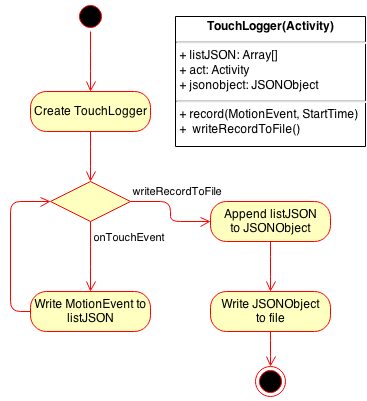
\includegraphics[scale=0.8]{TouchLogger.png}
\subsubsection{Resurser}
Kravet är att det finns en viss mängd minne för datafilen som genereras. Eftersom det rör sig om en textfil blir den aldrig speciellt stor.
\subsubsection{Referenser}
Denna komponent bygger på klassen MotionEvent.
\url{http://developer.android.com/reference/android/view/MotionEvent.html}
\subsubsection{Process}
Vid initiering av en activity skapas ett TouchLogger-objekt. 
\begin{verbatim}
TouchLogger tl;
\end{verbatim}
I onCreate()-metoden initieras TouchLogger-objektet med parametern \textbf{this}.
\begin{verbatim}
tl = new TouchLogger(this);
\end{verbatim}
Parametern \textbf{this} är activity:n som skickas med. Detta krävs för att sedan kunna skriva datan till en textfil. \\
För att sedan påbörja inspelning av rörelsehändelser kallas metoden record(MotionEvent event, float startTime). Metoden kallas från onTouchEvent(MotionEvent event) vilken är inbyggd i Android. Metoden kallas när den aktiva activity:n registrerar ett MotionEvent. 
\begin{verbatim}
if (recording) {
    tl.record(event, startTime);
}
\end{verbatim}
Event är den rörelsehändelse som ska spelas in och startTime är tidpunkten för inspelningens start. Denna tidpunkt behövs för att ge nyttig information (Såsom hur långt in i inspelningen denna rörelsehändelse ska dyka upp).

 För att avsluta inspelningen kallas metoden
 \begin{verbatim}
 tl.writeRecordToFile();
 \end{verbatim}
 vars syfte är att skriva datan till en textfil som sedan kan laddas upp till servern.
\subsubsection{Data}
Komponenten skapar ett JSON-objekt som sedan skriver detta objekt till en textfil vilken levereras till servern. Exempel hur filen kan se ut:
\begin{verbatim}
{``events'':
	``[{``timestamp'':''200'',interval=''17'',action=''down'',index=''0'',''x''=''310'',y=''670''},
	     {``timestamp'':''217'',interval=''17'',action=''move'',index=''0'',''x''=''320'',y=''680''},
	     {``timestamp'':''234'',interval=''17'',action=''up'',index=''0'',''x''=''330'',y=''700''}]''
}
\end{verbatim}